\documentclass{beamer}
\usefonttheme[onlymath]{serif}
\usepackage{graphicx, hyperref}
\hypersetup{colorlinks, urlcolor=blue}
\usepackage{subcaption}
\usetheme{Boadilla}

\newcommand{\pvec}[1]{\vec{#1}\mkern2mu\vphantom{#1}}

\title{Wave Properties of Particles}
\author{Amey Joshi}
\date{\today}

\begin{document}
\begin{frame}
\titlepage
\end{frame}

\begin{frame}
\frametitle{de Broglie waves}
\begin{enumerate}
\item Experimental evidence strongly favoured treating waves as particles. Yet
people reluctantly accepted that view.
\item On the other hand, imagining wave properties in particles was a giant leap
of imagination. People warmed up to it surprisingly quickly.
\item Planck proposed $E = h\nu = hc/\lambda$ while Einstein inferred that 
$E=pc$. de Broglie combined the two
\begin{equation}\label{e1}
\frac{hc}{\lambda} = pc \Rightarrow \lambda = \frac{h}{p}.
\end{equation}
A particle with momemtum $p$ has a `wavelength' $\lambda$.
\item Recall that $h = 6.626 \times 10^{-34}$ Js. An electron with mass $9.1
\times 10^{-31}$ kg and travelling with a speed $v = 1$ ms${}^{-1}$ will have
wavelength of the order of $10^{-3}$ m which is $1$ mm. What's your wavelength?
\end{enumerate}
\end{frame}

\begin{frame}
\frametitle{Cross with relativity?}
\begin{enumerate}
\item The momentum of a particle is $p = \gamma mv$ while energy is $E = \gamma
mc^2$. Therefore, $\lambda = h/p$ and $\nu = E/h$ give the velocity
\begin{equation}\label{e2}
v_p = \nu\lambda = \frac{E}{h}\times\frac{h}{p} = \frac{c^2}{v} > c.
\end{equation}
\item What exactly is $v_p$? How different is it from $v$? What does a velocity
greater than $c$ mean?
\item To answer this question we must examine the two ideas of phase and group
velocity.
\end{enumerate}
\end{frame}

\begin{frame}
\frametitle{Phase and group velocities}
\begin{enumerate}
\item The equation of a sinusoidal wave is
\begin{equation}\label{e3}
y = A\cos(kx - \omega t),
\end{equation}
where $k = 2\pi/\lambda$ is the wave number, $\omega = 2\pi/T = 2\pi\nu$ is the
angular frequency and $A$ is the amplitude. The ratio $\omega/k$ is called the
phase velocity. 
\item It is the speed at which a point of constant phase travels.
\item Consider a superposition of two waves $y_1 = A\cos(kx-\omega t)$ and $y_2
= A\cos[(k+\delta k)x - (\omega+\delta\omega)t]$. That is, we consider the wave
\begin{equation}\label{e4}
y = y_1 + y_2 = 2A\cos\left(\frac{\delta k}{2}x - \frac{\delta\omega}{2}t\right)
\cos(kx - \omega t)
\end{equation}
\item $y$ is a wave with modulated amplitude. The modulation travels at speed
$\delta\omega/\delta k$. The group velocity is this ratio as $\delta k
\rightarrow 0$.
\end{enumerate}
\end{frame}

\begin{frame}
\frametitle{Group velocity of de Broglie waves}
For de Broglie waves,
\begin{equation}\label{e5}
k = \frac{2\pi}{\lambda} = \frac{2\pi}{h}p = \frac{2\pi}{h}\gamma mv,
\end{equation}
so that
\begin{equation}\label{e6}
\frac{dk}{dv} = \frac{2\pi}{h}\frac{m}{(1 - \beta^2)^{3/2}}.
\end{equation}
Likewise,
\begin{equation}\label{e7}
\omega = 2\pi\nu = \frac{2\pi}{h}E = \frac{2\pi}{h}\gamma mc^2,
\end{equation}
so that
\begin{equation}\label{e8}
\frac{d\omega}{dv} = \frac{2\pi}{h}\frac{mv}{(1 - \beta^2)^{3/2}}.
\end{equation}
From \eqref{e6} and \eqref{e8}, $v_g = d\omega/dk = v$. The phase velocity has
no physical significance; the group velocity is the velocity of the particle.
\end{frame}

\begin{frame}
\frametitle{An experimental proof}
\begin{enumerate}
\item de Broglie waves are such that their group velocity matches the particle's
velocity. Is there an experimental proof for their existence?
\item `Light travels in a straight line', much like particles without any force 
on them, we learn in geometrical optics. But that does not tell why a shadow 
has a dark umbra and a lighter penumbra.
\item Diffraction is a property of waves. Penumbra is caused by diffraction.
\item Diffraction grating is a glass plate with finely etched lines spaced 
closely to make optical wavelength diffract.
\item Crystals act like gratings for X-rays. X-ray diffraction is well-
established technique to elucidate crystal structure.
\item Davisson and Germer showed that crystals also cause electrons to diffract.
Later on, diffraction was carried out by neutrons as well.
\end{enumerate}
\end{frame}

\begin{frame}
\frametitle{de Broglie waves, waves of what?}
\begin{enumerate}
\item Water waves involve oscillatory motion of water. Sound waves are a series
of compressions and rarefactions in a material. Electromagnetic waves involve
variation in electric and magnetic fields at a point. What oscillates in a de
Broglie wave?
\item de Broglie waves are called matter waves. If $\Psi(\vec{r}, t)$ is a 
function that characterises a matter wave then $|\Psi|^2$ is the probability
density function of finding a particle.
\item The probability of finding a particle in a small volume element $dV$
around a point $\vec{r}$ is proportional to $|\Psi|^2 dV$.
\item The quantity $\Psi$ is called a wave function; it is, in general, a 
complex-valued quantity. The `wave equation' of de Broglie waves is the 
Schr\"{o}dinger equation. 
\end{enumerate}
\end{frame}

\begin{frame}
\frametitle{The uncertainty principle}
\begin{enumerate}
\item Let's stay away from philosophy and just learn to calculate.
\item $|\Psi|^2$ is a probability distribution function. This indicates that we
can only predict the probability of a particle being in a neighbourgood of a 
point at a time $t$.
\item The position of a particle is a random variable. It has a mean, a variance
and higher moments. The square root of variance is called the uncertainty. It
is the same as standard deviation in statistics. In physics, we denote it as
$\Delta x$.
\item We will now see a few waves and visually examine the relation between 
our knowledge of $x$ and $k$.
\end{enumerate}
\end{frame}

\begin{frame}
\frametitle{Wave packets}
\begin{figure}
\begin{subfigure}{0.4\textwidth}
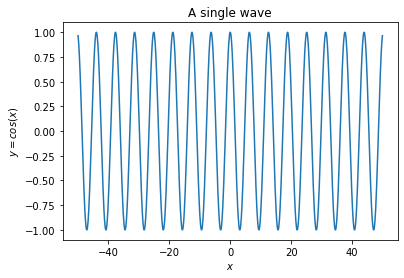
\includegraphics[scale=0.3]{one-wave}
\end{subfigure}
\hfill
\begin{subfigure}{0.4\textwidth}
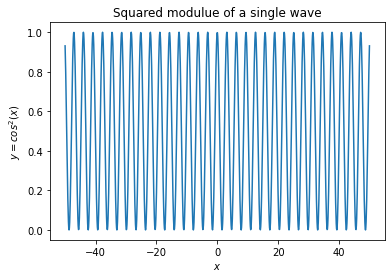
\includegraphics[scale=0.3]{one-wave-sq}
\end{subfigure}
\medskip
\begin{subfigure}{0.4\textwidth}
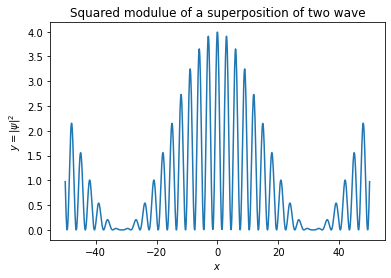
\includegraphics[scale=0.3]{two-waves-sq}
\end{subfigure}
\hfill
\begin{subfigure}{0.4\textwidth}
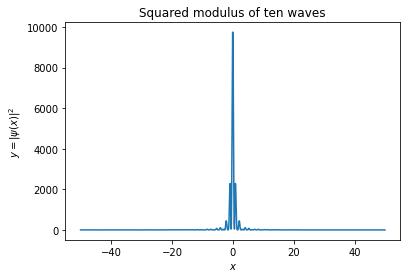
\includegraphics[scale=0.3]{ten-waves-sq}
\end{subfigure}
\end{figure}
\end{frame}

\begin{frame}
\frametitle{Wave packets}
\begin{enumerate}
\item For a single wave, $k$ is known with great precision but we have little
information about the particle's position.
\item With a superposition of two waves, we can tell the position of the 
particle with a little greater confidence at the cost of lesser precision in
the knowledge of $k$.
\item When we add ten waves together, we lose considerable information about $k$
but can point to the particle's position with far greater confidence.
\item Using Fourier transforms one can show that 
\begin{equation}\label{e9}
\Delta x \Delta k \ge \frac{1}{2}
\end{equation}
\item Physics tells us that $p = hk/(2\pi)$ so that 
\begin{equation}\label{e10}
\Delta x \Delta p \ge \frac{h}{4\pi}
\end{equation}
\end{enumerate}
\end{frame}
\end{document}